\subsection{Halfspaces}
\label{sec:halfspaces}
We will introduce hyperplanes, halfspaces and talk about their geometric properties. We will see that they are convex and have rather strong intersection properties. Later, we will introduce strongly separated halfspaces, which will be linked directly to the irreducibilty of a CAT(0) cube complex (see Proposition~\ref{prop:cs-5.1}). Lastly, we will be concerned with some combinatorial properties of halfspaces. The first part of this section follows the lecture notes by \textcite{Rolli2012}.

\begin{defin}[Hyperplanes]
  Let \(X\) be a cube complex.
  \begin{itemize}
  \item The 0-, 1- and 2-dimensional cubes are called \emph{vertices, edges} and \emph{squares} respectively.
  \item We say that two edges \(e\) and \(e'\) are equivalent (\(e \sim e'\)) if and only if either \(e' = e\) or there is a sequence of edges \(e_1, \dots, e_n\) such that \(e_1 = e\) and \(e_n = e'\) and any two edges \(e_{i-1}, e_i\) are opposite edges in a common square in \(X\). Note that this is an equivalence relation and we will call it \emph{square relation}.
  \item A midcube \(M \subset X\) is \emph{transverse} to a square relation class \(E = [e]_\sim\) (write \(M \pitchfork E\)) if \(M \cap X^{(1)}\) contains only midpoints of edges in \(E\).
  \item The \emph{hyperplane} defined by \(E\) is given by
    \begin{align*}
      \mathfrak{\hat h}(E) \coloneqq \bigcup_{M \pitchfork E} M \subset X.
    \end{align*}
    We will often write \(\mathfrak{\hat h}\) instead of \(\mathfrak{\hat h}(E)\).
  \end{itemize}
\end{defin}

\begin{bsp}
  Figure~\ref{fig:hyperplanes} contains an example of a CAT(0) cube complex with an equivalence class of edges (dark blue) and associated hyperplane (light blue). 
  \begin{figure}[htbp]
    \centering
    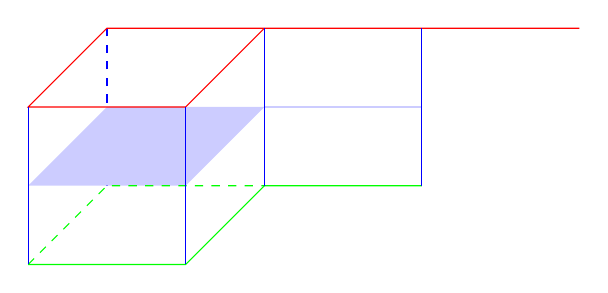
\begin{tikzpicture}
  [scale=2]
  \draw[blue,dashed] (0.5,0.5) -- (0.5,1.5);
  \fill[blue!20] (0, 0.5) -- (1, 0.5) -- (1.5, 1) -- (0.5, 1) -- (0, 0.5);
  \draw[blue!20] (1.5,1) -- (2.5,1);
  \draw[red] (1.5, 1.5) -- (1,1) -- (0,1) -- (0.5,1.5) -- (1.5,1.5) -- (2.5,1.5)  -- (3.5,1.5);
  \draw[green] (2.5,0.5) -- (1.5,0.5) -- (1,0) -- (0,0);
  \draw[green,dashed] (0,0) -- (0.5,0.5) -- (1.5,0.5);
  \draw[blue] (0,0) -- (0, 1)
  (1,0) -- (1,1)
  (1.5,0.5) -- (1.5,1.5)
  (2.5,0.5) -- (2.5,1.5);
\end{tikzpicture}

%%% Local Variables:
%%% mode: latex
%%% TeX-master: "../Master"
%%% End:

    \caption{Example of a CAT(0) cube complex with a hyperplane inscribed. The dark blue edges form an edge equivalence class, which defines the blue hyperplane. The red and green parts indicate the two halfspaces associated to the hyperplane. The figure follows closely the example in \textcite{sageev-lecture-notes}.}
    \label{fig:hyperplanes}
  \end{figure}
\end{bsp}

\begin{prop}[Convexity of halfspaces,\ {\cite[Propositions 18 \& 19]{Rolli2012}}]
  Let \(X\) be a CAT(0) cube complex and \(\mathfrak{\hat h} \subset X\) a hyperplane. Then \(\mathfrak{\hat h}\) is closed and convex. Furthermore, if \(\mathfrak{\hat h}\) contains at least two points of the image of any geodesic \(\gamma\), then the whole image of \(\gamma\) is contained in \(\halfspace{\hat h}\).
\end{prop}

\begin{cor}
  Let \(X\) be a CAT(0) cube complex. Every \(\mathfrak{\hat h} \subset X\) is itself a CAT(0) cube complex.
\end{cor}

\begin{proof}[Sketch]
  By construction, it is easy to verify that the gluing of midcubes inherited from \(X\) gives \(\mathfrak{\hat h}\) a cube complex structer. Additionally, every convex closed subspace of a CAT(0) space is CAT(0) itself.
\end{proof}

\begin{thm}[Separation, {\cite[Proposition 21]{Rolli2012}}]
  Any hyperplane \(\mathfrak{\hat h}\) separates \(X\) in exactly two convex connected components.
\end{thm}

\begin{defin}[Halfspaces]
  The two connected components of \(X \setminus \mathfrak{\hat h}\) are called \emph{halfspaces}. If \(\halfspace{h} \subset X \setminus \mathfrak{\hat h}\) is one of these halfspaces, then \(\halfspace{h}^\ast\) denotes the opposite halfspace leading to \(X = \halfspace{h}\, \sqcup\, \mathfrak{\hat h}\, \sqcup\, \halfspace{h}^\ast \).
\end{defin}

\begin{bsp}
  Figure~\ref{fig:hyperplanes} also indicates the two halfspaces (red and green color).
\end{bsp}

\begin{thm}[Intersection, {\cite[Proposition 22 \& 24]{Rolli2012}}]~\vspace{-6pt}
  \label{thm:common-intersection}
  \begin{enumerate} 
  \item Let \(\mathfrak{\hat h}_1, \dots, \mathfrak{\hat h}_n\) be hyperplanes with pairwise non-trivial intersection. Then
    \begin{align*}
      \bigcap_{i=1}^n \mathfrak{\hat h}_i \neq \varnothing.
    \end{align*}
  \item Let \(\halfspace{h}_1, \dots, \halfspace{h}_n\) be halfspaces with pairwise non-trivial intersection. Then
    \begin{align*}
      \bigcap_{i=1}^n \halfspace{h}_i \neq \varnothing.
    \end{align*}
    In particular, the intersection contains a vertex of \(X\).
  \end{enumerate}
\end{thm}

This concludes our discussion of geometric properties. The following definition will play a central role in Section~\ref{sec:group} (see for example Proposition~\ref{prop:cs-5.1}).

\begin{defin}[Strongly separated halfspaces]
  \label{defin:strong-sep}
  Two hyperplanes are \emph{strongly separated} if they are parallel (i.\,e.\ they do not intersect) and there is no hyperplane transverse to both. Two halfspaces are \emph{strongly separated} if the same is true for their associated hyperplanes.
\end{defin}

\begin{bsp}[Euclidean space]
  The space \(\R^d\) with its standard cubulation is one example of a CAT(0) cube complex \emph{without} any strongly separated hyperplanes. Indeed, any pair of parallel hyperplanes is orthogonal to some coordinate axis. Any hyperplane parallel to this axis is transverse to both.
\end{bsp}
\begin{bsp}[A tree]
  As an example \emph{with} strongly separated halfspaces, consider the tree depicted in Figure~\ref{fig:str-sep}. There we have three pairwise parallel hyperplanes \(\mathfrak{\hat h}, \mathfrak{\hat k}\) and \(\mathfrak{\hat l}\). Hence, any pair is strongly separated.

  \begin{figure}[htbp]
    \centering
    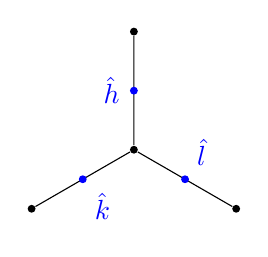
\begin{tikzpicture}
    [
  vertex/.style={
    circle,
    fill=black,
    minimum size=1mm,
    inner sep=0pt
  },
  hp/.style={
    circle,
    fill=blue,
    minimum size=1mm,
    inner sep=0pt
  },
  ->-/.style={
    decoration={
      markings,
      mark=at position 0.5 with {\arrow{#1}}
    },
    postaction={decorate}
  },
  scale=1.5
  ]
  \node (0) at (0,0) [vertex] {};
  \node (1) at (090:1) [vertex] {};
  \node (2) at (210:1) [vertex] {};
  \node (3) at (330:1) [vertex] {};
  \draw (0) -- (1)
  (0) -- (2)
  (0) -- (3);
  \node at (090:0.5) [hp,label={[blue]180:\(\mathfrak{\hat h}\)}] {};
  \node at (210:0.5) [hp,label={[blue]300:\(\mathfrak{\hat k}\)}] {};
  \node at (330:0.5) [hp,label={[blue]420:\(\mathfrak{\hat l}\)}] {};
\end{tikzpicture}
%%% Local Variables:
%%% mode: latex
%%% TeX-master: "../Master"
%%% End:

    \caption{A tree with three pairwise parallel hyperplanes \(\mathfrak{\hat h}, \mathfrak{\hat k}\) and \(\mathfrak{\hat l}\).}
    \label{fig:str-sep}
  \end{figure}
\end{bsp}

We close this section with two technical results. The first one will be employed in the metrizability of the Roller compactification (see Corollary~\ref{cor:comp-met}). The significance of the second result will become clear in Proposition~\ref{prop:pocset-halfspaces} and Remark~\ref{rem:roller}.

\begin{cor}
  \label{cor:halfspace-countable}
  If \(X\) is a locally countable CAT(0) cube complex, then its set of hyperplanes \(\mathcal{\hat H}\) and its set of halfspaces \(\mathcal{H}\) are countable.
\end{cor}

\begin{proof}
  We fix a vertex \(x_0 \in V(X)\) and consider the sets
  \[
    Y_n \coloneqq \{(x,y) \in X_{n-1} \times X_{n} \mid y \in N(x)\} \subset X_{n-1} \times X_n \quad \forall n \in \N.
  \]
  By Lemma~\ref{lem:lf-countable}, the sets \(X_n\) are countable and we have that
  \[
    \mathcal{\hat H} = \bigcup_{n=1}^\infty \bigcup_{e \in Y_n} \mathfrak{\hat h}([e])
  \]
  is countable. Since every hyperplane has exactly two halfspaces associated to it, the same is true for \(\mathcal{H}\).
\end{proof}

\begin{lemma}
  \label{lem:finite-interval}
  Let \(X\) be a connected CAT(0) cube complex. Then for any two \(\mathfrak{h,k} \in \mathcal{H}(X)\) such that \(\mathfrak{h} \subset \mathfrak{k}\) we have
  \[
    |\{\mathfrak{l} \in \mathcal{H}(X) \mid \mathfrak{h} \subset \mathfrak{l} \subset \mathfrak{k}\}| < \infty.
  \]
\end{lemma}

\begin{proof}
  Let \(M\) be the set as in the statement above and \(\hat M\) the set of corresponding hyperplanes. Clearly, the two sets are one-to-one. We take any vertex \(v \in \mathfrak{h}\)  and \(w \in \mathfrak{k}^\ast\). Then there exists a finite edge path \(c\) joining the two. We claim that \(\hat M\) is a subset of all the hyperplanes defined by the edges in \(c\). Indeed, let \(\mathfrak{l} \in M\). Then \(v \in \mathfrak{l}\) and \(w \in \mathfrak{l}^\ast\). Hence, \(c\) has to cross \(\mathfrak{\hat l}\). So \(\mathfrak{\hat l}\) is one of the hyperplanes defined by an edge in \(c\).
\end{proof}

%%% Local Variables:
%%% mode: latex
%%% TeX-master: "../Master"
%%% ispell-local-dictionary: "en_US"
%%% End:
